\section{Deep Learning Architectures \label{archi}}
We now turn our attention to the DL models that we have developed to help predict molecular properties.
\subsection{Overview}
    \begin{figure}[htbp]
        \centering
        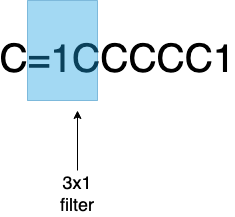
\includegraphics[width=0.15\textwidth]{figures/convonsmiles.png}
        \caption{A 3x1 filter in a 1-D Conv scanning a SMILES string. }
        \label{fig:conv-filter}
    \end{figure}
The main idea in our effort is to apply DL methods to the SMILES string to learn meaningful patterns from the atoms and bonds. This knowledge should help create models that predict molecular properties from first principles and without explicitly encoding rules from chemistry. Figure \ref{fig:conv-filter} shows this idea in the context of a 1-D Convolutional Neural Networks (1-D Convs). In this figure, a $3 \times 1$ filter is used to scan the string and find patterns in the sequence of atoms and bonds. This filter moves over the string looking at groups of three characters at a time and shifting one character to the right to look for the next group. Indeed, the figure depicts the second movement of the filter; the first movement covered the sub-string ``C=1".  In practice, however, this filter does not run directly over the characters of the string but instead  over the {\em character-level embeddings}  of the SMILES string. This approach will be explained in section \ref{embeddings}


In this paper, we shall focus on the use of 1-D Convs as the core methods used to build our models. Our work is still early, and we have also experimented with LSTM networks and Transformers. However,  1-D Convs have so far provided us with the best tradeoff between training speed and prediction error. Comparing all these various methods in detail is part of our future work and is therefore outside the scope of this paper. 


    
Figure \ref{fig:ml-framework} shows the end-to-end machine learning framework that we propose. We start out with a sample of the data from PubChem that contains 600,000 examples. We follow the standard practice of splitting this data set into training, validation and test sets. During the training phase, the training data is fed as tensor input to the model. Next, a character-level embedding layer takes care of mapping the characters in the SMILES string into an $n$-dimensional vector space. These transformed data are then passed through several 1-D Conv layers to build and detect features in the SMILES strings. Later on, the tensors generated in these layers are ``flattened" from their multi-dimensional shapes and fed into fully-connected layers, with the last layer producing the predictions of the model.
    \begin{figure}[htbp]
        \centering
        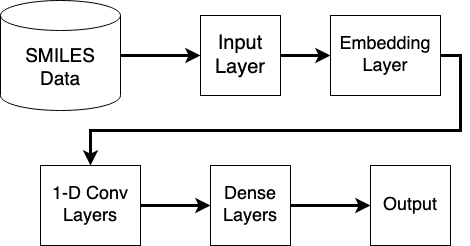
\includegraphics[width=0.4\textwidth]{figures/1DConvArch.png}
        \caption{Proposed end-to-end machine learning framework.}
        \label{fig:ml-framework}
    \end{figure}
\subsection{Character-level Embeddings \label{embeddings}}
DL models expect their input as tensors, and the SMILES strings are not. Hence, we need a method to represent SMILES in tensor form. In the context of NLP, word embeddings and character-level embeddings have become the preferred way to accomplish this, replacing one-hot encodings and bag-of-words models. The reason for this  is that embeddings can retain the information about relationships, context, and meaning that exists between adjacent words or characters. Thus, embeddings provide a dense representation of words, characters, and their
meaning within a sentence. 

In our work we do not use word embeddings but rather character-level embeddings (REF). This is mainly because the structure of the SMILES does not map to the concept of sentences separated by spaces as is the case for regular language sentences. Also, character level embeddings solve the {\em out-of-vocabulary (OOV) words} issue that often plagues word embedding methods.

  \begin{figure}[htbp]
        \centering
        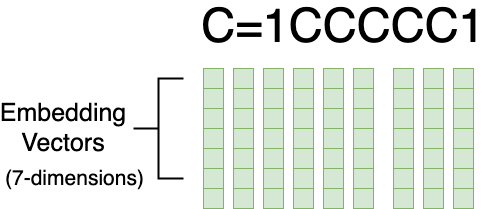
\includegraphics[width=0.4\textwidth]{figures/smileembedding.png}
        \caption{Embedding representation of a SMILES string.}
        \label{fig:smiles-to-embed}
    \end{figure}
Figure \ref{fig:smiles-to-embed} depicts a SMILES string and a  character-level embedding in a 7-D vector space. Each character is mapped to a vector with 7 dimensions, and each component in such vector is a real number.  In practice, this vector space can have a high dimension, with some models reported in the literature using a dimension of 256. Finding the right dimension size is still much of an experimental issue. This SMILES  string in 
Figure \ref{fig:smiles-to-embed} can then be represented as  a $9 \times 7$ matrix, with each row being a transposed embedding vector.
The standard practice in DL is to threat the embedding as  another layer in the neural work that can be trained to find the right values for the weights that produce the vectors. Some methods allow {\em pre-training} these weights on a very large corpus representative of the target data set, and then load them to form  a pre-trained embedding layer in the model. This form of {\em transfer learning} enables researchers to benefit from these pre-trained embeddings  and 
 focus on the design and tuning of the followup layers (i.e., the layers for the ``downstream task").

    % Model descriptions
    \subsection{Deep Learning to Predict Molecular Weight from SMILES}
    The first task that we discuss is the prediction of the molecular weight in a molecule. This is a baseline task since the molecular weight can be estimated as the sum of the weights in all the atoms in the molecule. Thus, our aim here is to determine if  a DL model, without any knowledge of chemistry or the periodic table, can learn to predict the molecular weight from the SMILES string. Thus, the first model that we will discuss is a DL model that receives a SMILES string as input and returns its prediction of the molecular weight. This model is shown in Figure \ref{fig:mw-architecture}.
    
        \begin{figure}[htbp]
        \centering
        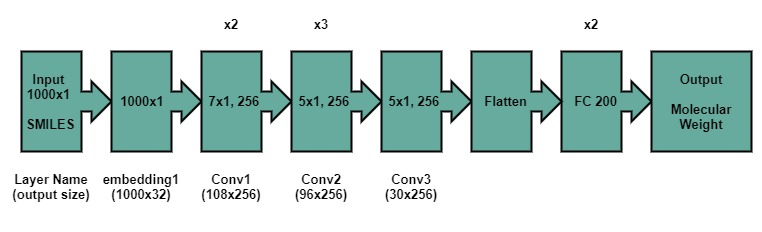
\includegraphics[width=0.5\textwidth]{figures/MW-model_arquitecture.jpg}
        \caption{The architecture of the model that predicts the molecular weight of a compound based on its SMILES string.}
        \label{fig:mw-architecture}
    \end{figure}
    This model  receives as input the pre-processed SMILES strings, capped at a maximum length of 1000 characters\footnote{Molecules found in PubChem can be rather large in size.}. Padding is used to make all SMILES string equal in size to 1000 characters. The embedding contains a vocabulary of 25 characters used to represents atoms, bonds, branches, etc. In order to feed the input to the neural network, we first transform each string into an array of the same length. Each entry 
    in this array is an integer representing the index of the character in the vocabulary. 
    
    The input layer of the network feeds the embedding layer, which maps strings into a  32-D vector space. This layer has an embedding matrix 
    of  $1000 \times 32$. The embedding is then passed to a sequence of six (6)  1-D Convs layers with 256 filters per layer. 
    In  our figures a symbol of $x2$ means that the same unit repeats twice, whereas $x3$ means that the same unit repeats three times. 
Notice that the first two convolutional layers are identical; they had a kernel of size 7x1 and were followed by 1-D max pooling of size 3.
The next three convolutional  layers had  kernels with size 3x1 and no pooling. The sixth convolutional layer had kernels of size 3x1 
and a 1-D max pooling layer of size 3. The result of the convolutions are then passed to a flatten layer, which in turn is passed to the final three dense layers. The first two dense layers consisted of 200 neural units and the final (output) one had only 1 neural unit. All of the dense layers had a ReLU activation function. The final  dense layer gives us the model's prediction of the molecular weight.

    
%        \begin{itemize}
%            \item The first model we will discuss is a DL model that receives an embedded SMILES string as input and as a result returns its prediction of the molecular weight. This model is shown in Figure \ref{fig:mw-architecture}.
%            \item Its architecture consisted first of a character embedding layer, that initially had random weights.
%            \item This layer receives as input the pre-processed SMILES strings that had a length of 1000 and vocabulary size of 25.
%            \item Its output is then passed to a 1D Convolutional Neural Network (CNN) that consists of 6 layers in total of 256 units each.
%            \item The first two convolutional layers had a kernel of size 7x1 and were followed by 1D max pooling of size 3.
%            \item The rest of the layers had kernels of size 3x1.
%            \item The final layer was also followed by 1D max pooling layer of size 3.
%            \item The result of the convolution was then passed to a flatten layer, which in turn is passed to the final three dense layers. 
%            \item The first two dense layers consisted if 200 units and the final had only 1 unit. 
%            \item All of the dense layers had a ReLU activation function.
%            \item The final dense layer gives us the model's prediction of the molecular weight.
%        \end{itemize}
    \subsection{Deep Learning to Predict XLogP from SMILES}
    The next task that we discuss is the prediction of the XLogP values from the SMILES strings. This task is more challenging than the previous one, and the interested reader can refer to (REF) for a discussion on the computational methods currently used  in practice to obtain 
    this quantity.  
    
    The  architecture of our second model can be seen in Figure \ref{fig:xlogp-archi1}. This architecture  is very similar to the one used for predicting the molecular weight. In fact, the input and embedding layers are the same. The difference consists in the units and the kernel sizes used in the convolutional and dense layers. The embedding layer is once again followed by six (6) 1-D Convs with 256 filters in each.
    The kernel sizes differ in this model; the first 2 convolutional layers have a kernel size of 5x1 and the kernel size for the remaining four (4)  is 3x1. A 1-D max pooling layer of size 3 is used after second and sixth 1-D Conv layers. The two (2) dense layers that follow the flatten layer 
    were changed with respect to the first model, and  now consist  100 and 200 neural units respectively. The final dense layer has one neural unit and gives us the model's prediction of the XLogP. As in the previous model for molecular weight, all dense layers used ReLU activation. 
    
        \begin{figure}[htbp]
        \centering
        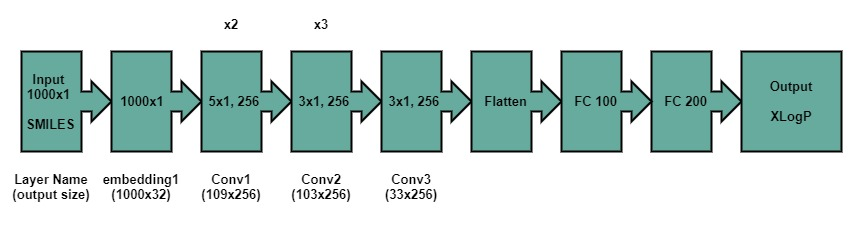
\includegraphics[width=0.5\textwidth]{figures/XLogP-model_arquitecture.jpg}
        \caption{The architecture of the model that predicts the XLogP of a compound based on its SMILES string.}
        \label{fig:xlogp-archi1}
    \end{figure}
  

%        \begin{itemize}
%            \item The architecture for the second model is similar to the one used for predicting the molecular weight.
%            \item The difference consists in the units and the kernel sizes used.
%            \item This model it also receives as input SMILES strings of length 1000 and vocabulary size of 25.
%            \item The embedding layer is once again followed by a CNN of 6 layers of 256 units each.
%            \item The kernel sizes differ in this model the first 2 convolutional layers have a kernel size of 5x1 and the kernel size for the rest is 3x1.
%            \item The 2 dense layers that follow now consist of 100 and 200 units respectively. 
%            \item Finally, the final dense layer gives us the models prediction of the XLogP.
%            \item The models architecture can be seen in Figure \ref{fig:xlogp-archi1}
%        \end{itemize}
    \subsection{Deep Learning to Predict XLogP from SMILES and fragments}
    The third and final task that we discuss is the prediction of XLopP from SMILES and chemical fragments. In this context, 
    fragments are molecules that result from simulated chemical transformations  that mimic  common reactions carried out in the lab to decompose a molecule into simpler parts. This decomposition can shed light into the functional structure and chemical properties of the molecule. The work in (REF) used this idea to explore word embeddings for functional chemical fragments 
    (i.e., fragments with well-known chemical properties). In our work, we used the open-source RDKit - Open-Source Cheminformatics Software   (REF) and RECAP method to create these fragments.
    
    Our model for this task is shown in Figure \ref{fig:xlogp-archi2}. This model differs from the previous two in that is receives two inputs: 1) the SMILES string for the original molecule and 2) a list of SMILES for the fragments of the molecule. Since for this model we have two sets of strings that we want it to use as input, we needed one embedding layer for each type of input received. One of the embedding layers receives the SMILES string for the molecule and the other receives the SMILES for the RECAP fragments of the molecule. In this instance
    the embeddings used a 57-D vector space. All the embeddings are then concatenated and supplied to the 1-D Conv layers that follow. 
    After the concatenation layer, the models follows the exact same setup as the model used for predicting molecular weight. The output from the final dense layer is the predicted XLogP of the chemical compound.  The final dense layer has one neural unit, and as before, all the dense layers use ReLU activation. 
    
%        \begin{itemize}
%            \item This model is similar to the first model, it differs in that it receives 2 inputs. 
%            \item The model's architecture is shown in Figure \ref{fig:xlogp-archi2}
%            \item Since for this model we have two sets of strings that we want it to use as input, we needed one embedding layer for each input received.
%            \item One of the embedding layers receives the SMILES strings and the other receives the RECAP fragments of the chemical compound.
%            \item These two embedding layers are then concatenated and supplied to the 1D CNN as input.
%            \item The CNN and fully connected layers used had the same setup as the first model that predicted molecular weight.
%            \item The output from the final dense layer is the predicted XLogP of the chemical compound.
%        \end{itemize}
    
    % Figures

  \begin{figure}[htbp]
        %\centering
        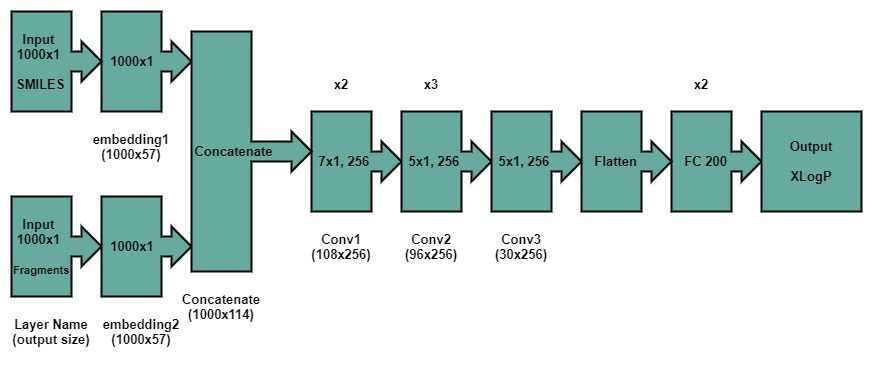
\includegraphics[width=0.5\textwidth]{figures/XLogP_frag_model_arquitecture.jpg}
        \caption{The architecture of the model that predicts the XLogP of a compound based on its SMILES string and RECAP fragments.}
        \label{fig:xlogp-archi2}
    \end{figure}